\subsection{Модели безопасности в СУБД}

Сегодня существует большое число различных теоретических моделей, которые позволяют описать практически все аспекты безопасности и обеспечивают средства защиты информации формально подтверждённой алгоритмической базой. Однако на практике воспользоваться результатами данных исследований не всегда удается, потому что слишком часто теория защиты информации не согласуется с реальной жизнью. Дело в том, что теоретические исследования в области защиты информационных систем носит разрозненный характер и не составляет комплексной теории. Существующие технические разработки основаны на различных подходах к проблеме, поэтому методы её решения существенно различаются. Наибольшее развитие получили два подхода -- это формальное моделирования политики безопасности и криптография. Эти различные по происхождению и решаемым задачам подходы взаимно дополняют друг друга. В отличии от криптографии, формальные модели безопасности предоставляют разработчикам защищенных систем принципы, которые лежат в основе архитектуры защищенной системы и определяют концепцию её построения.

Под \textit{политикой безопасности} понимается совокупность норм и правил, определяющих меры по обеспечению безопасности даанных, обрабатываемых в информационной системе.  Для реализации политики безопасности, сформулированной в терминах естест­венного языка, необходимо представить ее формальное выражение.  Его называют \textbf{модель политики безопасности} (или просто \textbf{модель безопасности}).

Далее мы разберем основные модели безопасности. Наиболее важные модели мы разберём подробно, а оставшиеся затронем кратко,  отослав заинтересованного читателя к первоисточникам.

\paragraph{Определения}

Перед дальнейшим расcмотрением моделей безопасности сформулируем основные определения:

\begin{itemize}
	\item Политика безопасности -- совокупность норм и правил, определяющих меры по обеспечению безопасности даанных, обрабатываемых в информационной системе.
	\item Модель безопасности -- формальное выражение политики безопасности.
	\item Монитор безопасности -- механизм реализации политики безопасности в автоматизированной системе, совокупность аппаратных, программных и специальных компонент системы, реализующих функции защиты и обеспечения безопасности (общепринятое сокращение -- Trusted Computing Base, TCB).
	\item Правила разграничения доступа -- совокупность правил, регламентирующих права доступа субъектов доступа к объектам доступа.
	\item Объект доступа -- единица информационного ресурса, доступ к которой регламентируется правилами разграничения доступа.
	\item Субъект доступа -- лицо или процесс, действия которого регламентируются правилами разграничения доступа.
	\item Состояние системы -- cовокупность множеств субъектов, объектов и отношений между ними. Каждое состояние системы является либо безопасным, либо небезопасным в соответствии с предложенными в модели критериями безопасности.
\end{itemize}

\paragraph{Основная теорема безопасности (Basic Security Theorem)}

Во время работы над моделью безопасности Белла-ЛаПадулы авторы пошли несколько дальше, и основываясь на формальном математическом аппарате, попытались строго доказать свойство защищенности своей модели. В результате они сформулировали и доказали "Основную теорему безопасности" (Basic Security Theorem):

\begin{grayquote}
Система безопасна тогда, и только тогда, когда ее начальное состояние безопасно, и любые переходы между ее состояниями также безопасны. Тогда и любое последующее состояние этой системы также будет безопасным, вне зависимости от обрабатываемой информации и конкретных процессов ее обработки.
\end{grayquote}

Теорема предполагает, что имеется возможность проверить безопасность начального состояния и всех возможных переходов состояний, чтобы доказать безопасность всей системы.

За моделью Белла-ЛаПадулы последовали другие модели управления доступом, создатели которых доказывали основную теорему безопасности и для них. Считалось, что доказательство этой теоремы доказывает безопасность и надежность самой модели.

Так продолжалось до середины 1980-х годов, когда Дж. Маклеан (J. McLean) подверг основную теорему безопасности критике. Маклеан предположил и обосновал, что она абсолютно бесполезна в силу своей тривиальности. Теорема никак не адресует собственно понятие безопасности, но демонстрирует общее свойство всех систем, допускающих формальное представление в виде конечного автомата с индуктивными переходами между последовательными состояниями. Безопасность же, скорее неформальное понятие.

После этого, попытки формального математического обоснования надежности и безопасности различных моделей управления доступом прекратились. Вопрос о возможности формализации и строгом математическом доказательстве свойства защищенности при обработке информации в вычислительной системе остается открытым до настоящего времени.

\subsubsection{Аспекты исследования моделей безопасности}

Основная цель создания и формального описания политики безопасности -- это определение условий, которым должно подчиняться поведение системы, выработка критерия безопасности и проведение формального доказательства соответствия системы этому критерию при соблюдении установленных правил и ограничений.

Исследование моделей безопасности выполняется с разных сторон. Можно выделить следующие аспекты:

\begin{itemize}
	\item Сущности системы -- субъекты и объекты.
	\item Возможные связи между сущностями системы.
	\item Разрешенные функции перехода между состояниями системы.
	\item Выполнение основной теоремы безопасности.
	\item Реализация монитора безопасности.
\end{itemize}

\subsubsection{Классификация моделей безопасности}

Обычно говоря о моделях безопасности имеют ввиду модели разграничения доступа. Различают три основные модели контроля доступа:

\begin{enumerate}
    \item\textbf{Дискреционная} (англ. discretionary access control, DAC);
    \item\textbf{Мандатная} (англ. mandatory access control, MAC);
    \item\textbf{Ролевая} (англ. role-based access control, RBAC).
\end{enumerate}

\subsubsection{Дискреционная модель}

Политика дискреционного управления достуом реализована в большинстве защищенных информационных систем и исторически является первой проработанной в теоретическом и практическом плане. Первые описания моделей дискреционного доступа появились еще в 60-х годах и подробно представлены в литературе.

На практике дискреционная модель доступа предполагает, что для каждого объекта в системе определен субъект-владелец. Этот субъект может самостоятельно устанавливать необходимые, по его мнению, права доступа к любому из своих объектов для остальных субъектов, в том числе и для себя самого. Логически владелец объекта является владельцем информации, находящейся в этом объекте.  При доступе некоторого субъекта к какому-либо объекту система контроля доступа лишь считывает установленные для объекта права доступа и сравнивает их с правами доступа субъекта. Кроме того, предполагается наличие в ОС некоторого выделенного субъекта -- администратора дискреционного управления доступом, который имеет привилегию устанавливать дискреционные права доступа для любых, даже ему не принадлежащих объектов в системе.

Кратко рассмотрим основные модели безопасности.

\paragraph{HRU}

Модель безопасности Харрисона-Руззо-Ульмана (HRU-модель) (середина 1970-х гг.) реализует произвольное управление
доступом субъектов к объектам и контроль за распространением прав доступа \autocite{Zegzhda}. Названа в честь
трёх его авторов: Майкла Харрисона, Уолтера Руззо и Джеффри Ульмана.

Главной особенностью является матрица доступа с полным описанием пользовательских прав к файлам. Изменения в эту
матрицу вводятся с помощью специальных команд.

\textbf{Представления модели.} Введем некоторые обозначения:
\begin{itemize}
    \item S — множество субъектов;
    \item O — множество объектов;
    \item R = (r\textsubscript{1}, r\textsubscript{2}, ... , r\textsubscript{n}) — множество прав доступа.
\end{itemize}
Для реализации этих прав в данной модели используется матрица доступов M, строки которой соответствуют субъектам,
а столбцы — объектам. На пересечении строчек и столбцов указаны права доступа R, которыми обладает данный субъект
по отношению к данному объекту. Тогда текущее состояние системы Q можно однозначно записать в таком виде:
Q = (S, O, M). Также вводят множество возможных операций A = (a\textsubscript{1}, a\textsubscript{2}, ... , a\textsubscript{k}).

\textbf{Критерий безопасности системы.} Для заданной системы исходное состояние Q\textsubscript{0} = (S\textsubscript{0},
O\textsubscript{0}, M\textsubscript{0}) называется безопасным относительно права r, если не существует такой
последовательности команд, которая изменила бы заданное начальное состояние системы так, что право r записалось бы в
ячейку M[s;o], в которой оно отсутствовало в начальном состоянии Q\textsubscript{0} \autocite{Zegzhda}. Если это условие не выполнено,
то произошла утечка информации.

\textbf{Определение.} Монооперационная команда -- команда, состоящая из не более чем одной элементарной операции \autocite{Zegzhda}.

\textbf{Определение.} Монооперационная система -- система, все команды которой являются монооперационными.

\textbf{Теорема.} Существует алгоритм, проверяющий на безопасность исходное состояние Q\textsubscript{0}
монооперационной системы на безопасность относительно права r \autocite{WikiHRU}.

\textbf{Теорема.} Задача определения безопасности исходного состояния Q\textsubscript{0} системы общего вида для
данного права r является неразрешимой \autocite{WikiHRU}.

Основным преимуществом модели над другими дискреционными является строгость критерия безопасности \autocite{WikiHRU}.

\paragraph{Take-Grant}

Несмотря на недостатки дискреционных моделей безопасности, относительно простая реализация их на практике побудила
исследователей к усовершенствованию моделей типа HRU, в которых проблема контроля распространения прав доступа
алгоритмически не разрешима \autocite{URFULecture10Models}.

Например, \textit{система передачи прав доступа встраивается в систему разграничения в виде дополнительных прав}, образуя
модель передачи прав доступа Take-Grant (1976). В этой модели доказывается безопасное состояние системы после
изменения прав доступа к объекту или субъекту путем преобразования графов доступа \autocite{URFULecture10Models}.

Модель представляет всю систему как направленный граф, где узлы — либо объекты, либо субъекты. Дуги между ними
маркированы, и их значения указывают права, которые имеет объект или субъект (узел). В модели доминируют два правила:
«брать» и «давать». Они играют в ней особую роль, переписывая правила, описывающие допустимые пути изменения графа \autocite{WikiTakeGrant}.
В общей сложности существует 4 правила преобразования:
\begin{itemize}
    \item правило «брать»;
    \item правило «давать»;
    \item правило «создать»;
    \item правило «удалить».
\end{itemize}
Используя эти правила, можно воспроизвести состояния, в которых будет находиться система в зависимости от распределения
и изменения прав доступа. Следовательно, можно проанализировать возможные угрозы для данной системы.

\textbf{Представления модели.} Введем некоторые обозначения:
\begin{itemize}
    \item S — множество субъектов;
    \item O — множество объектов;
    \item R = (r\textsubscript{1}, r\textsubscript{2}, ... , r\textsubscript{n}) -— множество прав доступа.
\end{itemize}

\textbf{Правило «брать».}
\begin{figure}[H]
    \centering
    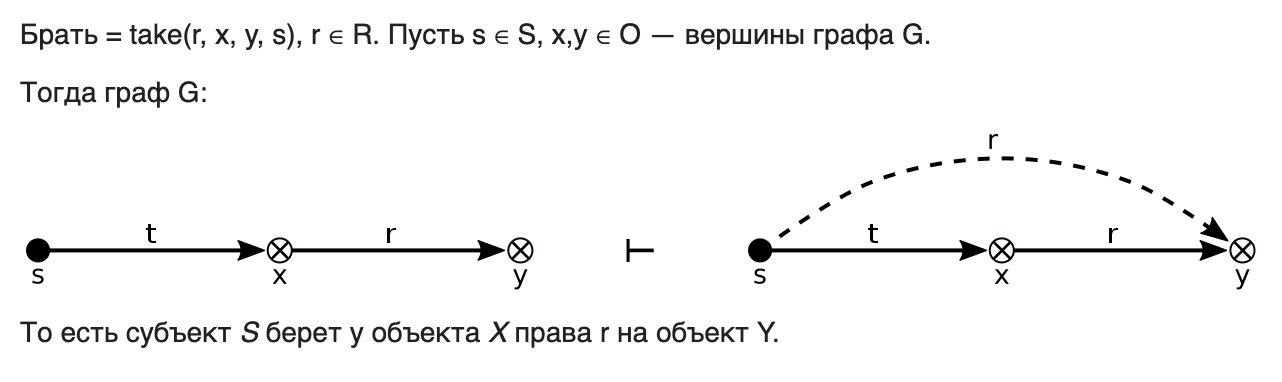
\includegraphics[width=0.8\textwidth]{assets/models/take_grant_bring.png}
\end{figure}

\textbf{Правило «давать».}
\begin{figure}[H]
    \centering
    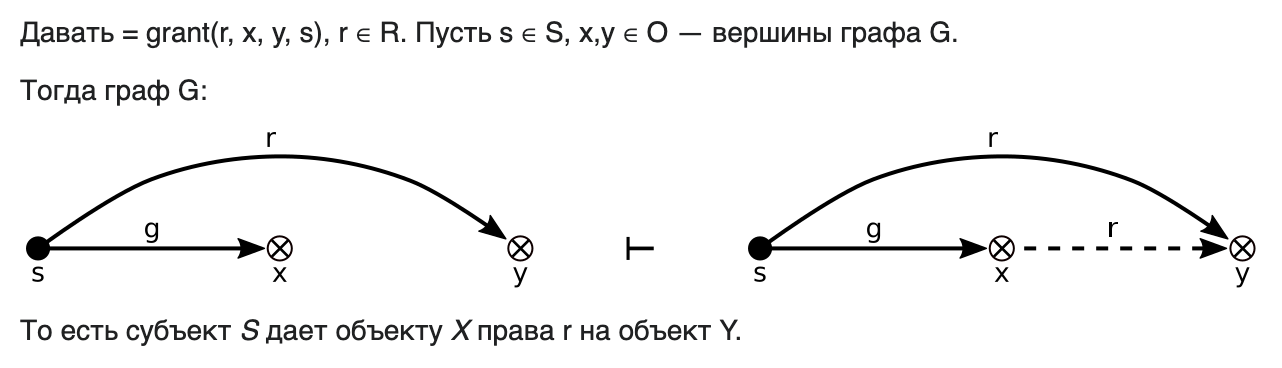
\includegraphics[width=0.8\textwidth]{assets/models/take_grant_give.png}
\end{figure}

\textbf{Правило «создать».}
\begin{figure}[H]
    \centering
    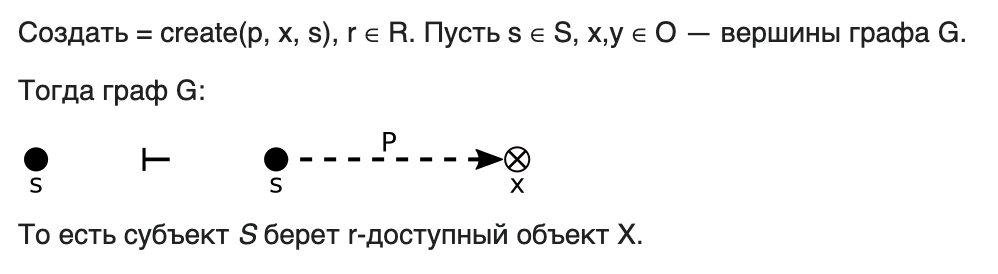
\includegraphics[width=0.8\textwidth]{assets/models/take_grant_create.png}
\end{figure}

\textbf{Правило «удалить».}
\begin{figure}[H]
    \centering
    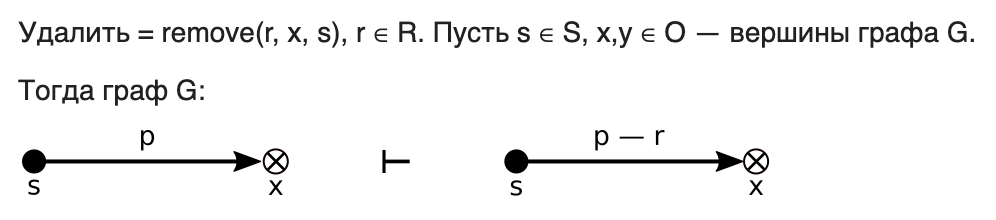
\includegraphics[width=0.8\textwidth]{assets/models/take_grant_delete.png}
\end{figure}

По-сути критерием безопасности системы при использовании модели Take-Grant является невозможность нарушения
прав доступа при выполнении установленных правил.

Результатом модели становится представление системы как направленного графа с дугами - правами между субъектами
и объектами.

Следующие две модели намного менее популярны, поэтому при их рассмотрении ссылаемся только на англоязычные
источники.

\paragraph{Action-Entity}

Модель Acten (Action Entity) была предложена Буссолати и др. \autocite{Jalili} в 1983 г. Является расширением
модели Take-Grant \autocite{SecModels}:
\begin{itemize}
    \item Дополнительные административные привилегии (использование, создание, удаление, ...)
    \item Предикаты авторизации -- условия, которые должны быть выполнены для предоставления доступа
    \item Представление с использованием двух графиков (один для авторизации для статических действий и один
    для авторизации для динамических действий)
\end{itemize}
Цели расширения \autocite{Jalili}:
\begin{itemize}
    \item Исправление неизбирательности админских привилегий
    \item Увеличение контроля над транспортным потоком
\end{itemize}

\textit{Каждый элемент системы, имеющий отношение к безопасности, рассматривается как \textbf{сущность (Entity)}} \autocite{Jalili}:
\begin{itemize}
    \item Сущность касается как субъектов, так и объектов
    \item Сущности -- это типы ресурсов
\end{itemize}

\textit{Выделяют два режима доступа -- \textbf{действия (Action)}} \autocite{Jalili}:
\begin{itemize}
    \item cтатический;
    \item динамический.
\end{itemize}

\textbf{Статические действия (режим доступа).} Их выполнение не изменяет аутентификацию и состояние системы.
Состоят из \autocite{SecModels}:
\begin{itemize}
    \item «Использование»: между пользователями, операторами и ресурсами ввода-вывода, приложениями, ...
    \item «Чтение»: для доступа к содержимому объекта
    \item «Написание» («Обновление»)
    \item «Создание»: сущностей
    \item «Удаление»: объекта
\end{itemize}

\textbf{Динамические действия (режим доступа).} Их выполнение изменяет аутентификацию и/или состояние системы.
Состоят из \autocite{SecModels}:
\begin{itemize}
    \item «Грант» (предоставить, Grant): удержание субъектом Ei статического режима m по отношению к Ek
    позволяет Ei предоставить субъекту Ej режим m на Ek
    \item «Отозвать»
    \item «Делегировать»: позволяет Ei предоставлять Ej динамическое разрешение на «грант», относящееся к режиму m
    на Ek. Авторизация для делегирования/отмены ограничена несколькими объектами
    \item «Отменить»
\end{itemize}

Вводится иерархия отношений между статическими режимами \autocite{Jalili}:
\begin{itemize}
    \item «Создание»/«Удаление» -- 4
    \item «Обновление» -- 3
    \item «Чтение» -- 2
    \item «Использование» -- 1
\end{itemize}

И между динамическими режимами (административными правами) \autocite{Jalili}:
\begin{itemize}
    \item «Делегировать»/«Отменить» -- 2
    \item «Грант»/«Отозвать» -- 1
\end{itemize}

В соответствии с этими иерархиями в модели Action Entity строят два графа:
\begin{itemize}
    \item cтатических режимов;
    \item динамических режимов.
\end{itemize}

Вводят определённые правила для двух графов, которые являются критерием безопасности системы \autocite{SecModels}.
Подробное изложение можно найти в \autocite{SecModels} и в \autocite{Jalili}.

\paragraph{Wood}

Единственным источником, где удалось найти хоть какую-то информацию о модели Woods является \autocite{Jalili}.
Согласно нему модель была разработана в 1979 г. Вудсом. Ориентация модели на управлении аутентификацией и контролем
доступа в БД многоуровневой схемы. Модель рассматривает трехуровневую модель ANSI / SPARC, включая:
\begin{itemize}
    \item Внешний уровень: ближайший к пользователю
    \item Концептуальный уровень: представление данных
    \item Внутренний уровень: ближайший к физическому хранению, не привязанный к аппаратным элементам.
\end{itemize}

Субъекты -- пользователи системы:
\begin{itemize}
    \item Авторизатор, который управляет авторизацией
    \item Пользователи, имеющие доступ к данным
\end{itemize}

Объекты -- объекты концептуального уровня: каждый O принадлежит к категории типа, заданной функцией n(O),
указывает свою категорию типа (n (O)):
\begin{itemize}
    \item Категории типов на концептуальном уровне: набор сущностей, тип отношения и атрибут
    \item Атрибут может быть связан с одним набором объектов и сопоставляет набор объектов с набором значений
    \item Тип отношения -- это двунаправленная ассоциация между двумя наборами сущностей и может иметь два имени
\end{itemize}

Cостояние авторизации указывается в правилах доступа. Правила доступа имеют вид <s, o, t, p>, где субъект s
реализует режим доступа t к объекту o при условии p. Правила доступа определяются авторизатором. Основные правила
указаны в концептуальном уровне, который представляет собой глобальное представление данных организации. Определение
таблицы (на внешнем уровне) включает ограничения доступа, определяющие, какие типы доступа допустимы для
каждый внешний объект e (каждая таблица и ее поля). Эти ограничения хранятся в ограничении доступа (Access Constraint, AC).

\subsubsection{Мандатная модель}

Приведём классическое определение мандатной модели из \textit{Оранжевой книги}.

\begin{grayquote}
Мандатная модель контроля доступа – это модель, в которой используются средства ограничения доступа к объектам,  основанные на секретности информации,  содержащейся в объектах, и обязательная авторизация действий субъектов для доступа к информации с присвоенным уровнем важности.
\end{grayquote}

Важность информации определяется уровнем доступа,  который приписываетя всем объектам и субъектам.  В сравнении с дискреционным мандатное управление доступом устанавливает гораздо более строгие правила определения прав доступа субъектов к объектам. Предполагается, что некоторый выделенный привилегированный субъект – администратор мандатного управления доступом – определяет необходимые, и согласованные с установленной в системе политикой безопасности, права доступа каждого из субъектов к каждому из объектов. Никакой другой субъект системы не может устанавливать или изменять свои, либо чьи-то еще права доступа к объектам. В такой системе права доступа пользователей определяются, прежде всего, интересами безопасности владельца всей системы.

Далее рассмотрим наиболее популярные мандатные модели безопасности.

\paragraph{Модель Белла-ЛаПадулы}

В середине 1970-х годов, два математика из MITRE Corporation -- Д. Белл (D. Bell) и Л. ЛаПадула (L. LaPadula) -- работая по проекту Министерства Обороны США, разработали мандатную модель, названную затем по их именам.

Основной задачей проекта была разработка и формальное обоснование модели управления доступом, функционально согласованную с методиками работы, принятым при обработке бумажной документации конфиденциального характера, т.е. имеющей грифы "секретно", "совершенно секретно" и т.п. Сложившаяся на тот момент практика обработки бумажной документации позволяла избежать несанкционированного доступа к информации, а также обладала приемлемой степенью удобства, поэтому было решено применить подобную схему и в вычислительной системе. Суть проекта состояла именно в этом. Интересно, что данный факт порой ускользает от внимания специалистов в области защиты информации.

Ниже дается упрощенное математическое описание модели Белла-ЛаПадулы.

Вычислительная система рассматривается в виде набора субъектов $S_{i}$, набора объектов $O_{j}$ и матрицы управления доступом $M[i*j]$.

Имеется набор упорядоченных уровней секретности -- иерархия уровней. Каждый субъект и каждый объект имеет назначенный ему \textit{индивидуальный уровень секретности}. Кроме того, каждый субъект имеет еще \textit{текущий уровень секретности}, который не может превосходить его индивидуальный уровень секретности. Таким образом, субъект может произвольно изменять свой текущий уровень секретности в диапазоне, не выше своего индивидуального уровня. Обычно используют четыре уровня секретности, каждый из которых доминирует над уровнем, находящиимся ниже в ииерархии: совершенно секретно ($top-secret$),  секретно ($secret$),  конфиденциально ($confidential$) и несекретно ($unclassified$).  При этом верно следующее: $ top-secret \supset secret \supset confidential \supset unclassified $.

Предполагается, что уровень секретности $S_1$ доминирует над уровнем $S_2$, если он больше или равен $S_2$, т.е. $S_1 \geq S_2$.

Функция всех возможных в системе взаимных уровней секретностей субъектов и объектов $F$ задается полным набором троек ($f_S(S_i)$ , $f_C(S_i)$, $f_O(O_j)$). Здесь $f_S(S_i)$ – индивидуальный уровень секретности субъекта $S_i$, $f_O(O_j)$ – индивидуальный уровень секретности объекта $O_j$, а $f_C(S_i)$ – текущий уровень секретности субъекта Si. Очевидно, что $f_S(S_i)$ должен доминировать над $f_C(S_i)$ для всех $S_i$. Рассматриваются четыре типа прав доступа субъекта к объекту:

\begin{enumerate}
	\item\textbf{только чтение} (read-only, ro) произвольных участков данных;
	\item\textbf{дополнение} (append, ad) - субъект может только записывать данные, размещая их в конце объекта;
	\item\textbf{исполнение} (execute, ex) - субъект не может ни читать, ни записывать данные объекта, но может исполнять этот объект, как прикладную программу;
	\item\textbf{чтение и запись} (read-write, rw) - субъект может и читать, и записывать данные объекта, по принципу произвольного доступа.
\end{enumerate}

Набор всех типов прав доступа обозначают $A$, а любой его элемент -- $x$.

Матрица управления доступом $M[i;j]$ содержит в каждой из своих ячеек $M_{ij}$ текущие дискреционные права доступа $x$ (поднабор из $A$) субъекта $S_i$ к объекту $O_j$. Каждый столбец матрицы составляет атрибут управления объекта $O_j$, и является совокупным набором текущих прав доступа к нему всех субъектов. Атрибут управления для объекта $O_j$ выдается субъекту $S_k$ во время создания им этого объекта. Таким образом, субъект-создатель может устанавливать и отменять текущие дискреционные права доступа для любых субъектов, в том числе и для себя самого. Для этого он модифицирует соответствующие ячейки столбца $M_j$ матрицы доступа $M[i;j]$, изменяя этим атрибут управления объекта $O_j$. Однако он не может передать право изменения атрибута управления какому-либо другому субъекту.

Всякое обращение субъекта $S_i$ к объекту $O_j$ с типом доступа x описывается тройкой ($S_i$ , $O_j$, $x$), а совокупность всех текущих обращений в системе -- набором доступов $b$.

Теперь всю систему защиты можно описать в виде автомата конечных состояний с набором функций перехода между состояниями. Состояние модели $z$ задается набором из четырех элементов ($b$, $M[i;j]$, $F$,  $O_j$). С течением времени система принимает некоторую последовательность состояний $z$, с начальным состоянием $z_0$.

Разрешены следующие функции перехода между состояниями:

\begin{enumerate}
	\item изменение набора текущих доступов $b$;
	\item изменение матрицы управления доступом $M[i;j]$;
	\item изменение набора объектов set $O_j$;
	\item субъект $S_i$ может изменять свой текущий уровень секретности, но не выше его индивидуального уровня секретности.
\end{enumerate}

Чтобы модель обеспечивала защиту, нужно чтобы всякий раз для функции перехода между состояниями удовлетворялся ряд дополнительных условий. Эти условия называется свойствами защиты.В модели Белла – ЛаПадулы устанавливаются и поддерживаются два мандатных и одно дискреционное свойства защиты\footnotemark:

\footnotetext{В англоязычной литературе первое свойство называют simple security property, а второе – *-property. }

\begin{enumerate}
    \item Субъект с определённым уровнем секретности не может иметь доступ на чтение объектов с более высоким уровнем секретности (англ. no read-up).
    \item Субъект с определённым уровнем секретности не может иметь доступ на запись объектов с более низким уровнем секретности (англ. no write-down).
    \item Использование матрицы доступа субъектов к объектам для описания дискреционного доступа.
\end{enumerate}

Описанные три свойства защиты в обязательном порядке реализуются в системе защиты. Также требуется, чтобы каждое из свойств обязательно удовлетворялось для любого состояния системы защиты. Такие состояния называются безопасными состояниями.

Свойства защиты служат лишь общей директивой для действующих правил управления доступом. Текущий доступ ($S_i$, $O_j$, $x$) может быть предоставлен только в том случае, если выполнены следующие условия:

\begin{enumerate}
	\item $ss-property$: $f_C(S_i)$ доминирует над $f_O(O_j)$, если $x = ro$ или $x = rw$.
	\item $*-property$:
	\begin{enumerate}
		\item $f_O (O_j)$ доминирует над $f_C(S_i)$, если $x = ad$.
		\item $f_O(O_j)$ равен $f_C(S_i)$, если $x = rw$.
		\item $f_C(S_i)$ доминирует над $f_O(O_j)$, если $x = ro$.
	\end{enumerate}
	\item $ds-property$: $x$ находится в ячейке $M_{ij}$ текущих прав доступа матрицы $M[i*j]$.
\end{enumerate}

\subparagraph{Недостатки модели Белла-ЛаПадулы}

Легко увидеть, что из описания модели Белла-ЛаПадулы нельзя определить формальных принципов назначения атрибутов безопасности субъектам и объектам. Действительно, в ней определены и обоснованы все правила управления доступом на основе атрибутов безопасности, но не способы их назначения при создании субъектов и объектов, импорте объектов в систему и т.д. Данный факт вызывает некоторые проблемы при практическом использовании модели.

Другим недостатком модели Белла-ЛаПадулы принято считать ее излишнюю строгость -- возможность передачи информации только в сторону увеличения ее уровня секретности: "write up - read down". Это не всегда совместимо с нормальным функционированием реальной вычислительной системы. В силу тех же причин, несколько субъектов с разным уровнем секретности не могут равноправно получать доступ к одному объекту, например, совместно использовать один принтер для вывода информации на печать. Для устранения описанных ограничений в реальных системных обычно реализуют доверенных субъектов или доверенные программы, которые являются посредниками, гарантирующими безопасность несогласованных с моделью видов доступа.

Еще одним основанием для критики модели является проблема скрытых каналов (covert channels). Суть ее в том, что большинство ресурсов вычислительных систем, в том числе операционных систем UNIX - машинное время, устройства хранения информации - совместно и равноправно используются субъектами. Ресурсы выделяются субъектам по мере необходимости. Это рационально, однако также позволяет двум различным субъектам по предварительной договоренности произвольно обмениваться информацией без учета правил управления доступом, заложенных в модели защиты. Например, один из субъектов моделирует ресурсы системы, усиливая и уменьшая вычислительную нагрузку на компьютер, или записывая и удаляя данные во внешней памяти. Это можно рассматривать как закодированную информацию, которую другой субъект считывает, измеряя периодически скорость выполнения своей задачи, или пытаясь также записать данные во внешнюю память.

Борьба со скрытыми каналами чрезвычайно трудна, так сами каналы являются следствием стремления к оптимальному использованию ресурсов системы. Обычно считается, что пропускная способность скрытых каналов слишком мала, и они не могут нанести серьезный ущерб безопасности. К тому же, они предполагают предварительный сговор двух субъектов, что маловероятно. Наличие скрытых каналов просто игнорируется, что можно в некоторой степени считать решением проблемы. В то же время, системы обработки особо конфиденциальной информации должны проектироваться с учетом проблемы скрытых каналов, возможно, в ущерб их производительности.

К числу недостатков модели Белла-ЛаПадулы также относят проблему целостности обрабатываемой информации, определяемую как невозможность искажения и/или уничтожения информации несанкционированными субъектами. Действительно, в рамках правил модели происходит передача информации в сторону повышения ее секретности. Однако разумно предположить, что менее секретная информация заслуживает меньшего доверия, равно как и менее секретный субъект, который может передать ее выше, исказив или уничтожив при этом конфиденциальные данные. Одновременно, с точки зрения системы, повышается (необоснованно) уровень доверия к передаваемой информации. То есть задача защиты информации в модели Белла-ЛаПадулы решается не полностью - конфиденциальная информация может быть искажена и даже уничтожена субъектом с низким уровнем секретности; хотя модель одновременно эффективно препятствует несанкционированному доступу к информации, ее утечке.

Целостность информации принято гарантировать реализацией в вычислительных системах специальных дополнительных моделей защиты. Дискреционное управление доступом также может обеспечить целостность информации в объекте, если его субъект-владелец позаботится об этом, установив соответствующие права доступа к нему.

Важно понимать, что сама по себе модель Белла-ЛаПадулы обладает рядом существенных недостатков, которые проявляются на практике. Тем не менее, она стала отправной точкой в области разработки мандатных моделей безопасности.

\paragraph{Модель Биба}

Модель Биба (англ., Biba model) оригинальным образом поддерживает целостность информации в системе, представимой в виде набора взаимодействующих субъектов и объектов. Она строится на основе иерархии уровней целостности (доверенности, достоверности) информации и двух основных правил ее обработки -- аксиом целостности:

\begin{itemize}
	\item аксиома простой целостности запрещает чтение информации более доверенным субъектом из менее достоверного объекта;
	\item аксиома целостности запрещает запись информации менее доверенным субъектом в более достоверный объект.
\end{itemize}

Таким образом, общие правила данной модели обозначить "no write up - no read down", что показывает ее логическую инверсию к модели Белла-ЛаПадулы.

Легко убедиться, что модель Биба позволяет решить проблемы поддержания целостности обрабатываемой информации и сохранения доверия к ней. Действительно, система запрещает произвольное повышение достоверности информации, более доверенные субъекты не могут пользоваться менее достоверной информацией, а общий уровень достоверности комплексной информации, находящейся в объекте, равен минимальному уровню достоверности ее составляющих.

Как модель Белла-ЛаПадулы, так и модель Биба, часто называют моделями информационных потоков (information-flow model), так как информация в вычислительной системе может перемещаться при обработке только в виде потоков, разрешенных в рамках модели: "write up - read down"; "no write up - no read down".

Таким образом, единственной проблемой модели Белла-ЛаПадулы, к решению которой не существует общего подхода, является определение принципов назначения атрибутов безопасности субъектам и объектам.

\paragraph{Модель Дион}

Предлагается в качестве обязательной политики, которая одновременно обеспечивает секретность и целостность.
Сочетает в себе принципы модели Биба (политика строгой последовательности). В модели нет дискреционной
политики. Не позволяет передавать информацию от объектов к субъектам (через операции записи). Поток данных
разрешен только между объектами, но никогда между объектами и субъектами. Содержит введение концепции связи между
объектами для обмена информацией между ними.

Субъекты -- это сущности, выполняемые в системе от имени пользователей. Каждому системному объекту назначается
3 уровня безопасности и 3 уровня целостности:
\begin{itemize}
    \item ASL (Absolute Security Level) указывается при создании и фиксируется на всю жизнь предмета. Это второй уровень
    пользователя, соответствующий теме
    \item RSL (Read Security Level) -- это самый высокий уровень безопасности, с которого субъекту разрешено читать
    \item WSL -- это самый низкий уровень безопасности, на который субъекту разрешено писать
    \item AIL (Absolute Integrity Level) присваивается при создании и фиксируется на всю жизнь субъекта. Это уровень
    целостности пользователя, соответствующий предмету
    \item RIL: самый низкий уровень целостности, с которого субъекту разрешено читать
    \item WIL: наивысший уровень целостности, на который субъекту разрешено писать.
\end{itemize}

Устанавливаются ограничения -- для каждого субъекта $s$:

\begin{center}
$WSL(s) \leqslant ASL(s) \leq RSL(s)$ \\
$RIL(s) \leqslant AIL(s) \leq WIL(s)$
\end{center}

Субъект для которого строго соблюдается хотя бы одно неравенство удовлетворенный считается доверенным. Субъект может
быть доверенным с точки зрения секретности, целостности или того и другого. Субъекты, для которых 4 отношения
удовлетворяются знаком равенства, считаются недоверенными.

Объекты -- любая сущность хранения данных в системе. Каждому объекту назначается 3 уровня безопасности и
3 уровня целостности:
\begin{itemize}
    \item ASL (Absolute sec level) -- уровень безопасности данных, содержащихся в объекте; фиксируется на весь срок
    службы объекта
    \item MSL (Migration sec level) -- это самый высокий уровень безопасности, на который могут передаваться данные
    в объекте
    \item CSL (Corruption sec level) - это самый низкий уровень безопасности, с которого данные могут поступать в объект
    \item AIL (Absolute int level) - это уровень целостности данных в объекте
    \item MIL (Migration int level) - это самый низкий уровень целостности, на который могут передаваться данные в объекте
    \item CIL (Corruption int level) - это самый высокий уровень целостности, с которого данные могут поступать в объект
\end{itemize}

Аналогично:

\begin{center}
$CSL(o) \leqslant ASL(o) \leq MSL(o)$ \\
$MIL(o) \leqslant AIL(o) \leq CIL(o)$
\end{center}

В модели вводится ряд дополнительных аксиом и правил на отношения между субъектами и объектами.

\paragraph{Многозначность в БД с многоуровневой секретностью}

Как уже было показано,  принципы модели безопасности Белла-ЛаПадулы сами по себе вполне здравые,  но на практике поддержание нескольких уровней защиты в пределах одной таблицы (или в одной базе данных) сопряжено с рядом серьезных проблем.  Рассмотрим, например, следующую ситуацию.

Сотрудник военного ведомства, чьи персональные данные хранятся в базе данных с многоуровневой защитой, может иметь "настоящую" миссию, например быть сотрудником отдела по борьбе с терроризмом, и в то же время некоторое "прикрытие", согласно которому он является, допустим, членом отряда десантников. При этом в базе данных должна быть представлена и реальная информация, и прикрытие.

Мы могли бы расширить модель безопасности, добавив свойство секретности не только для каждой строки, но и на уровне элементов. Но это расширение приведет к новым серьезным проблемам, поскольку каждый элемент в строке может принимать одно из нескольких возможных значений, в зависимости от уровня доступа субъекта. Такое положение дел на фундаментальном уровне нарушает один из важнейших принципов реляционных баз данных – требование первой нормальной формы (1NF)\footnotemark.

\footnotetext{
Таблица считается приведенной к первой нормальной форме, если выполняются следующие условия:
\begin{itemize}
	\item В таблице не должно быть дублирующихся строк;
	\item В каждой ячейке таблицы должно храниться атомарное значение (одно не составное значение);
	\item В столбце должны храниться данные одного типа;
	\item Не должно быть массивов и списков.
\end{itemize}
}

Решение проблемы поэлементной классификации основано на идее многозначности --  когда в рамках одной таблицы может существовать множество записей с одним и тем же значением первичного ключа, но разными полями.  Многозначность впервые была применена в 1988 г. в модели безопасной базы данных SeaView (Secure Data Views).

\paragraph{SeaView}

Модель SeaView (Secure Data View) \autocite{SeaView} была предложена Дороти Деннинг в 1987 г. Она состоит из мандатной, дискреционной моделей, а также вспомогательной для добавления и классификации новой информации поступающей в базу данных. SeaView состоит из двух слоев:

\begin{itemize}
    \item \textbf{MAC}
    обязательный контроль доступа. Этот уровень соответствует обязательной политике безопасности моделей Bell-LaPadula и Biba.
    \item \textbf{Trusted Computing Base (TCB)}
    определяет концепцию многоуровневых отношений, поддерживает дискреционные средства управления для многоуровневых отношений и представлений, а также формализует поддерживающие политики.
\end{itemize}

Класс доступа в модели SeaView состоит из:

\begin{itemize}
    \item \textbf{Уровень секретности} -- иерархический уровень секретности.
    \item \textbf{Классы целостности} -- набор неирархических классов,между которыми определены отношения вложенности.
\end{itemize}

В рамках модели MAC каждому субъекту и объекту назначаются классы:

\begin{itemize}
    \item Класс для записи
    \item Класс для чтения
\end{itemize}

Причем для каждого объекта класс чтения должен быть выше класса записи. Субъект считается доверенным, если его класс чтения строго больше класса записи. Для недоверенных субъектов классы чтения и записи равны.

В рамках модели TCB реализуется многоуровневость.  Модель TCB определяет политику дискреционного управления доступом и поддерживающие политики. Она определяет компоненты многоуровневой защищенной системы реляционной базы данных, включая многоуровневые отношения, представления, ограничения целостности и дискреционные полномочия. Информация в модели TCB секретна и должна храниться в объектах, доступ к которым огранчен.

SeaView представляет собой набор одноуровневых БД.  Одноуровневые БД связанны с конкретным классом доступа. Таким образом, для реализации модели SeaView могут использоваться обыкновенные реляционные базы данных. А доступ к ним осуществляет отдельное ПО~--- монитор безопасности.  Он при попытке доступа субъекта к объекту сранивает классы доступа и принимает решение~--- разрешить действие или нет. Оригинальная статья формулирует следующее требование к монитору безопасности~--- он должен быть легковесным и легкопроверяемым на уязвимости. Требование подкрепляется ссылкой на Оранжевую книгу и объясняется тем, что монитор безопасности ключевой элемент, отвечающий за безопасность данных в модели SeaView.

\paragraph{Jajodia\&Sandhu}

Модель Джаджодиа–Сандху является производной от модели SeaView. Она модифицирует алгоритм, который разлагает
многоуровневое отношение на одноуровневые фрагменты, а также модифицирует алгоритм восстановления, который
восстанавливает исходное многоуровневое отношение \autocite{Osama}.

В модели Джаджодиа–Сандху алгоритм декомпозиции использует только горизонтальную фрагментацию, поскольку
вертикальной фрагментации не требуется. Это приводит к улучшению алгоритма восстановления в модели Джаджодиа–Сандху
по сравнению с алгоритмом восстановления в модели SeaView, поскольку можно восстановить многоуровневое отношение
без необходимости выполнять операции соединения; для восстановления многоуровневого отношения требуются только
операции объединения \autocite{Osama}.

В модели Джаджодиа–Сандху есть две основные проблемы \autocite{Osama}:
\begin{itemize}
    \item Семантическая неоднозначность: предположим, что есть два кортежа в отношениях с уровнями безопасности
    U и S, и нет кортежа с уровнем безопасности TS. Если пользователю с уровнем безопасности TS необходимо
    получить информацию из отношения, он не может решить, какая информация является правильной, потому что
    значения из кортежа U и кортежа S в отношении будут извлечены в результате запроса
    \item Операционная неполнота: предположим, что существует два несравнимых уровня безопасности, M1 и M2,
    наименьшая верхняя граница которых соответствует уровню безопасности S, а наибольшая нижняя граница --
    уровню безопасности U. Пользователь с уровнем безопасности S не может вставлять кортежи, которые содержат
    атрибуты с уровнями безопасности U, M1 и M2
\end{itemize}

\paragraph{Smith\&Winslett}

В модели Смита–Уинслетта многоуровневая реляционная база данных рассматривается как набор обычных реляционных
баз данных, в которых все базы данных используют одну и ту же схему. Эта модель не поддерживает безопасность
на уровне каждого отдельного атрибута. Уровень безопасности может быть назначен только атрибутам первичного
ключа и кортежам в целом \autocite{Osama}.

Многоуровневая реляционная схема задается как R($A_{pk}$, $C_{pk}$, $A_1$, ..., $A_{n}$, $T_C$), где $A_{pk}$ обозначается как атрибут данных первичного ключа, $C_{pk}$ - атрибут классификации первичного ключа, который содержит уровень безопасности первичного ключа. Атрибут данных $A_{1} ... A_{n}$ обозначается как атрибуты данных, а $T_C$ обозначается как атрибут классификации кортежа, который содержит уровень безопасности кортежа \autocite{Osama}.

Согласно этим правилам определяется доступ для обновления и чтения. Модификация базы данных (вставка, удаление
и обновление) пользователем может изменить данные только на уровне безопасности пользователя. Запрос от пользователя
с уровнем безопасности $L$ может получить доступ к данным именно из тех баз данных, уровень которых не выше уровня $L$
\autocite{Osama}.

В этой модели была добавлена семантика, основанная на концепции веры. Модель Смита–Уинслетта также известна как
модель семантики, основанная на убеждениях, а также представила концепцию базового кортежа. Базовый кортеж --
это самый низкий уровень безопасности кортежа базы данных, в котором утверждается существование объекта.
Таким образом, процедура обновления устраняет проблемы, присутствующие в модели Джаджодиа–Сандху, но ограничивает
объем обновления одним объектом \autocite{Osama}.

\paragraph{Решеточная}

Управление доступом на основе решеток (Lattice-Based Access Control, LBAC) - это сложная модель управления доступом,
основанная на взаимодействии между любой комбинацией объектов (например, ресурсов, компьютеров и приложений) и
субъектов (таких как отдельные лица, группы или организации) \autocite{LBAC}.

В этом типе модели управления принудительным доступом на основе меток решетка используется для определения уровней
безопасности, которые может иметь объект и к которым субъект может иметь доступ. Субъекту разрешен доступ к объекту
только в том случае, если уровень безопасности субъекта больше или равен уровню безопасности объекта \autocite{LBAC}.

Математически уровень безопасности доступа также может быть выражен в терминах решетки (набор частичного порядка),
где каждый объект и субъект имеют наибольшую нижнюю границу (совпадение) и наименьшую верхнюю границу (соединение)
прав доступа. Например, если двум субъектам A и B требуется доступ к объекту, уровень безопасности определяется как
соответствие уровней A и B. В другом примере, если два объекта X и Y объединены, они образуют другой объект Z,
которому присваивается уровень безопасности, образованный объединением уровней X и Y \autocite{LBAC}.

LBAC также известен как ограничение управления доступом на основе меток (или управление доступом на основе правил)
в отличие от управления доступом на основе ролей (RBAC) \autocite{LBAC}.

Модели управления доступом на основе решетки были впервые формально определены Деннингом (1976).

\subsubsection{Ролевая модель}

Ролевые модели безопасности нельзя отнести ни к дискреционным, ни к мандатным моделям, потому что
управление доступом в них осуществляется как на основе матрицы прав доступа для ролей, так и с помощью
правил, регламентирующих назначение ролей пользователям и их активации во время сеансов. Поэтому
ролевая модель представляет собой совершенно особый тип политики, основанный на компромиссе между
гибкостью и простотой управления доступом (характерным для дискреционных моделей), так и жёсткостью
правил контроля доступа (соответствующие мандатным моделям).

В ролевой модели классическое понятие \textit{субъект} заменяется понятиями \textit{пользователь} и
\textit{роль}. Пользователь -- это человек, работающий c системой и выполняющий определённые
обязанности. Роль -- это активно действующая в системе абстрактная сущность, c которой связан
ограниченный, логический связный набор полномочий, необходимый для осуществления определённой деятельности.

Такой подход в политике безопасности позволяет учесть разделение обязанностей и полномочий между
участниками прикладного информационного процесса, так как с точки зрения ролевой политики имеет
значение не личность пользователя, осуществляющего доступ к информации, а то какие полномочия ему
необходимы для выполнения его служебных обязанностей \autocite{Zegzhda}.

В качестве критерия безопасности ролевой модели используется следующее правило \autocite{Zegzhda}:
\textit{система считается безопасной, если любой пользователь системы, работающий в определённом
сеансе S, может осуществлять действия, требующие полномочия P только в том случае, если P принадлежит
разрешениям S.}

\subsubsection{Особенности реализации моделей безопасности в СУБД}

Почти все крупные производители СУБД ограничиваются развитием концепции конфиденциальности, целостности
и доступности данных, а их действия направлены, в основном, на преодоление существующих и уже известных
уязвимостей, реализацию основных моделей доступа и рассмотрение вопросов, специфичных для конкретной СУБД.
Такой подход обеспечивает решение конкретных задач, но не способствует появлению общей концепции
безопасности для такого класса ПО, как СУБД. Это значительно усложняет задачу по обеспечению безопасности
хранилищ данных на предприятии.

Обычно пользователей СУБД (субъектов) можно разделить на три группы, что влияет на применение определённых
моделей безопасности (разграничения доступа) \autocite{CitForumSafeDB}:
\begin{itemize}
    \item Прикладные программисты -- отвечают за создание программ, использующих базу данных. Программист
    может быть как пользователем, имеющим права создания и управления объектами (данными), так и пользователем,
    имеющим права только управления данными

    \item Конечные пользователи базы данных -- работают с БД непосредственно через терминал или рабочую станцию.
    Как правило, конечные пользователи имеют строго ограниченный набор прав управления данными. Этот набор
    может определяться при конфигурировании интерфейса конечного пользователя и не изменяться. Политику
    безопасности в данном случае определяет администратор безопасности или администратор БД (если это одно и
    то же должностное лицо)

    \item Администраторы баз данных -- образуют особую категорию пользователей СУБД. Они создают сами БД,
    осуществляют технический контроль функционирования СУБД, обеспечивают необходимое быстродействие системы.
    В обязанности администратора, также входит обеспечение пользователям доступа к необходимым им данным,
    написание (или оказание помощи в определении) необходимых пользователю внешних представлений данных.
    Администратор определяет политику безопасности
\end{itemize}

Отметим, что в настоящее время для контроля доступа в СУБД как правило используются дискреционные и ролевые
модели. Мандатные модели значительно менее популярны в силу ряда недостатков в их использовании в СУБД.

\paragraph{Дискреционные и ролевые модели доступа}

При использовании дискреционных моделей в СУБД:
\begin{itemize}
    \item Субъект -- системный идентификатор, от имени которого СУБД выполняет определенные действия над
    определенными объектами. Понятие субъекта отличается от понятия пользователь компьютерной системы,
    поскольку инициировать изменение информации могут также и системные процессы
    \item Объект защиты -- часть БД, на которую распространяется действие конкретного правила безопасности;
    это может быть группа отношений, отдельное отношение, подмножества атрибутов и т.д.
    \item Привилегия -- действие над объектом защиты, которое может быть совершено от имени конкретного
    идентификатора (по сути элемент из множества отношений между субъектами и объектами -- право на доступ)
\end{itemize}

Чаще всего владельцем базы данных является Администратор БД. Ему предоставлены все системные и объектные
привилегии. В частности, он имеет право регистрации новых пользователей и предоставления им привилегий, как
системных, так и объектных. Пользователь, имеющий системные привилегии, является владельцем всех созданных им
объектов, имеет по отношению к ним все привилегии и может предоставлять их полностью или частично другим
пользователям. Минимальной системной привилегией является право подключения к СУБД - привилегия входа
\autocite{Skakun}.

Пользователи могут быть объединены в специальные группы пользователей. Один пользователь может входить в
несколько групп. Для пользователей с минимальным стандартным набором прав вводится понятие группы PUBLIC.
По умолчанию предполагается, что каждый вновь создаваемый пользователь, если специально не указано иное,
относится к группе PUBLIC (как минимум в PostgreSQL).

Привилегии конкретному пользователю могут быть назначены администратором явно и неявно, например, через роль.
Роль - это еще один возможный именованный носитель привилегий. Существует ряд стандартных ролей, которые
проектируются при разработке СУБД. Также имеется возможность создавать новые роли, группируя в них произвольные
полномочия. Введение ролей позволяет упростить управление привилегиями пользователей, структурировать этот
процесс. Кроме того, введение ролей не связано с конкретными пользователями, поэтому роли могут быть определены
и сконфигурированы до того, как определены пользователи системы.

\textbf{Операторы SQL предоставления и отмены привилегий.} В стандарте SQL определены два оператора GRANT и
REVOKE для предоставления и отмены привилегий соответственно. \textit{\textbf{Оператор предоставления привилегий}}
имеет следующий формат \autocite{Skakun}:
\begin{lstlisting}[]
GRANT {<action list>|ALL PRIVILEGES} ON <object name>
    TO {<user list>|PUBLIC} [WITH GRANT OPTION];
\end{lstlisting}
, где:
\begin{itemize}
    \item <action list>(<список действий>) определяет набор действий из доступного списка действий над объектом
    данного типа (параметр ALL PRIVILEGES указывает, что разрешены все действия, допустимые для объектов данного
    типа),
    \item <object name>(<имя объекта>) определяет имя объекта защиты: таблицы, представления, хранимой
    процедуры или триггера,
    \item <user list>(<список пользователей>) определяет список идентификаторов пользователей, кому предоставляются
    данные привилегии. Вместо списка идентификаторов можно воспользоваться параметром PUBLIC.
\end{itemize}
Параметр WITH GRANT OPTION является необязательным и определяет режим, при котором передаются не только права
на указанные действия, но и право передавать эти права другим пользователям. Передавать права в этом случае
пользователь может только в рамках разрешенных ему действий. В общем случае набор привилегий зависит от
реализации СУБД (определяется производителем). Выделяются привилегии манипулирования данными:
\begin{itemize}
    \item SELECT –- просматривать данные;
    \item INSERT [(<список полей>)] -– добавлять данные;
    \item UPDATE [(<список полей >)] -– обновлять данные;
    \item DELETE –- удалять данные;
    \item REFERENCES [(<список полей >)] -- ссылаться на указанные поля при определении ссылочной целостности;
    \item USAGE –- использовать домены и ограничители целостности;
    \item EXECUTE –- выполнять сохраненные процедуры и функции.
\end{itemize}
Среди привилегии создания/изменения объектов БД выделим наиболее часто используемые:
\begin{itemize}
    \item CREATE <тип объекта> -- создание объекта некоторого типа;
    \item ALTER <тип объекта> -- изменение структуры объекта;
    \item DROP <тип объекта> -- удаление объекта;
    \item ALL -- все возможные действия над объектом.
\end{itemize}

Для отмены ранее назначенных привилегий в стандарте SQL определен оператор REVOKE. \textit{\textbf{Оператор отмены
привилегий}} имеет следующий синтаксис \autocite{Skakun}:
\begin{lstlisting}[]
REVOKE {<action list>|ALL PRIVILEGES} ON <object name>
    FROM {<user list>|PUBLIC} {CASCADE|RESTRICT};
\end{lstlisting}
Параметры CASCADE или RESTRICT определяют, каким образом должна производиться отмена привилегий. Параметр
CASCADE отменяет привилегии не только пользователя, который непосредственно упоминался в операторе GRANT при
предоставлении ему привилегий, но и всем пользователям, которым этот пользователь присвоил привилегии,
воспользовавшись параметром WITH GRANT OPTION.

\textit{Дискреционная модель является очень популярной у разработчиков СУБД. Она реализована в практически всех
SQL-совместимых СУБД. Операторы SQL GRANT, REVOKE, DENY, реализующие дискреционную модель разграничения
доступа, определены в стандарте языка SQL.}

\textbf{Ролевая модель в СУБД.} Рассмотренная дискреционная модель в СУБД очень похожа на ролевую модель.
Основное отличие ролевой модели в СУБД -- это обязательное использование принципа наименьших привилегий
и то, что после авторизации пользователя в системе для него создается сессия. При реализации ролевой
модели может быть введен ряд ограничений \autocite{Skakun}: например, назначение роли главного администратора
(суперпользователя) может быть предоставлено только одному пользователю, вводится запрет совмещения одним
пользователем определенных ролей, ограничивается количество пользователей, одновременно выполняющих определенную
роль и т.п.

К недостаткам ролевого разграничения доступа в СУБД относится отсутствие формальных доказательств безопасности
компьютерной системы, возможность внесения дублирования и избыточности при предоставлении пользователям прав
доступа и сложность конструирования ролей \autocite{Skakun}.

Наряду с дискреционной, ролевая модель разграничения доступа, реализована во множестве развитых коммерческих
СУБД, например: Microsoft SQL Server, Oracle, IBM DB2 \autocite{Skakun}.

\paragraph{Мандатные модели доступа в СУБД}

Обычно мандатную модель доступа в СУБД реализуют с помощью модели Белл-ЛаПадула, о которой мы поговорим позже
при рассмотрении конкретных примеров мандатных моделей.

Перечислим основные недостатки применения мандатных моделей доступа в СУБД \autocite{Skakun}:
\begin{itemize}
    \item Невозможность автоматизации назначения уровней секретности и определения границ защищаемых данных,
    что в больших системах может приводить к практически бесконечному ручному процессу конфигурации системы
    \item Снижение эффективности работы компьютерной системы, так как проверка прав доступа субъекта к объекту
    выполняется не только при открытии объекта в процессе субъекта, но и перед выполнением любой операции
    чтения из объекта или записи в объект
    \item Создание дополнительных неудобств в работе пользователей компьютерной системы, связанных с
    невозможностью изменения информации в неконфиденциальном объекте, если тот же самый процесс использует
    информацию из конфиденциального объекта (его уровень конфиденциальности больше нуля). Это зачастую
    решается путем разрешения пользователю выступать от имени субъекта с меньшим уровнем доступа, что в
    свою очередь приводит к деградации системы защиты.
\end{itemize}

\textit{Из-за отмеченных недостатков мандатного разграничения доступа в реальных СУБД множество объектов, к которым
применяется мандатное разграничение, является подмножеством множества объектов, доступ к которым осуществляется
на основе дискреционного разграничения.}

Примером реализации мандатного подхода разграничения доступа можно считать компонент Oracle Label Security (OLS),
реализованный в СУБД Oracle, начиная с 9 версии. Примером Российской СУБД, реализующей стандарт SQL-92 является
СУБД ЛИНТЕР \autocite{Skakun}.

\subparagraph{Проблемы реализации многозначности}

Даже если отвлечься от проблемы хранения в базе данных разного рода легенд и прикрытий, многозначность все равно должна стать неотъемлемым свойством баз данных с многоуровневой защитой. Порассуждаем, каким образом следовало бы обрабатывать отношение с многоуровневой защитой в отсутствие многозначности. База данных может скрывать значения, недоступные пользователю или процессу по соображениям безопасности, и такое маскирование обычно осуществляется при помощи пустых значений (null values).

Напомним, что каждый кортеж существует в единственном экземпляре, поэтому непривилегированный процесс может попытаться записать неклассифицированные данные в столбцы кортежа, содержащие как бы пустые значения. В связи с этим в СУБД с многоуровневой защитой возникает проблема обработки таких операций, поскольку на самом деле значение столбца непустое, и замещать его нельзя. Естественно, что подобные попытки должны отвергаться средствами системы безопасности.

Однако неудача при выполнении операции модификации открывает определенные возможности, получившие название косвенных каналов (для получения закрытой информации), т. е. пути для снижения классификации данных (преднамеренного или случайного). Отказ в выполнении вроде бы вполне законной транзакции на модификацию пустых значений в базе данных с многоуровневой защитой выдает информацию о том, что эти элементы на самом деле не пусты, а содержат классифицированные данные. Уведомляя пользователя или процесс, не наделенных соответствующими полномочиями, о наличии скрытых данных в некотором кортеже, мы тем самым открываем косвенный канал.

Допустим, что СУБД с многоуровневой защитой симулирует выполнение подобных модификаций, чтобы не раскрывать скрытый канал. Если пользователь, только что изменивший некоторые данные, попытается обратиться к ним, ему ответят, что они отсутствуют. Тогда мы опять создаем косвенный канал.

А что если попытаться поддерживать в СУБД с многоуровневой защитой нечто вроде журнала таких модификаций и использовать его для последующих выборок? Знакомая идея, и неудивительно -- ведь мы только что говорили о многозначности. Даже если мы предусмотрим какое-нибудь специфическое решение для реализации многозначности, например хранить два экземпляра кортежей, -- это всего лишь одна из реализаций. Важно, что многозначность -- это существенное свойство данных с многоуровневой защитой, а как она будет реализована -- это вопрос второстепенный, не имеющий отношения к самой идее по-разному представлять информацию для пользователей разных уровней благонадежности; хотя способы реализации многозначности остаются важным направлением для исследовательской работы.

Рассматривая проблему реализации многозначности, полезно обратить внимание на концептуальное сходство между многозначными кортежами в базе данных с многоуровневой защитой и кортежами с множественными значениями в хронологических базах данных. Напомним, что в большинстве реляционных баз данных с расширениями для поддержки хронологизма должны существовать несколько экземпляров одного кортежа с одним и тем же значением первичного ключа, чтобы обеспечить отображение и текущего состояния объекта, и исторической информации о нем. В реляционной СУБД с расширениями для поддержки многоуровневой защиты по существу присутствует такой же тип представления с той разницей, что определяющим признаком экземпляров некоторого кортежа в хронологической базе данных является время, а в базе данных с многоуровневой защитой -- класс доступа. Хотя с других точек зрения, помимо реализации многозначности, хронологические СУБД и СУБД с многоуровневой защитой имеют мало общего, в связи с коммерциализацией СУБД обоих типов может оказаться полезным применять в них общие алгоритмы представления и доступа к многозначным кортежам.

Итак, многозначность, примененная впервые в проекте SeaView, стала общепринятой моделью реализации баз данных с многоуровневой защитой, в особенности реляционных. Многозначность активно исследуется и в качестве механизма обеспечения безопасности в объектно-ориентированных базах данных (развитие средств защиты в СУБД этого типа пока еще значительно отстает по сравнению с реляционными СУБД, но их значение будет неуклонно расти вместе со стремлением позиционировать ООСУБД на рынке продуктов для коммерческих и правительственных организаций).
